% fig-attack.tex: the rollback attack as run, as a timeline (draft of 5 Nov 2026, from section 3.5 and Table 3.3).
% Build from this folder:  pdflatex fig-attack.tex
% The adversary holds only the storage credential: it never sees a passphrase and never contacts the key server.
\documentclass[tikz,border=4pt,11pt]{standalone}
% style.tex: what the four diagrams share (colours, fonts, the look of a party, a message, a note).
% The one accent colour is the blue of the latency charts; it always means "the head", the thing this thesis adds.
% Everything else is black or grey, so the figures still read when printed in black and white.
\usepackage[T1]{fontenc}
\usepackage{mathptmx}
\usetikzlibrary{positioning,calc,arrows,fit,backgrounds}
\definecolor{head}{HTML}{2A78D6}
\definecolor{ink}{HTML}{0B0B0B}
\definecolor{inktwo}{HTML}{52514E}
\definecolor{soft}{HTML}{F0EFEC}
\definecolor{rule}{HTML}{C3C2B7}
\tikzset{
  every picture/.style={font=\small, >=latex},
  party/.style={draw=ink, fill=soft, rounded corners=2pt, minimum width=3.4cm, minimum height=0.8cm, align=center, font=\small\bfseries},
  box/.style={draw=ink, fill=soft, rounded corners=2pt, minimum width=3.9cm, minimum height=1.9cm, align=center},
  quiet/.style={draw=rule, text=inktwo},
  life/.style={draw=rule, line width=0.9pt},
  msg/.style={->, draw=ink, line width=0.7pt},
  rep/.style={->, draw=ink, line width=0.7pt, dashed},
  hmsg/.style={->, draw=head, line width=1.2pt},
  hrep/.style={->, draw=head, line width=1.2pt, dashed},
  bad/.style={->, draw=ink, line width=1.2pt, dashed},
  lab/.style={font=\footnotesize, inner sep=3pt, text=ink},
  act/.style={font=\footnotesize, align=left, text=ink, fill=white, draw=rule, rounded corners=1.5pt, inner sep=3pt},
  outcome/.style={font=\footnotesize, align=center, text=ink, fill=white, draw=ink, rounded corners=1.5pt, inner sep=4pt},
  side/.style={font=\footnotesize\itshape, align=left, text=inktwo},
  band/.style={fill=soft, draw=rule, rounded corners=2pt, minimum height=0.7cm, font=\footnotesize, text=inktwo},
  holds/.style={font=\footnotesize, text=inktwo, fill=white, draw=rule, rounded corners=1.5pt, inner sep=2.5pt},
}

\begin{document}
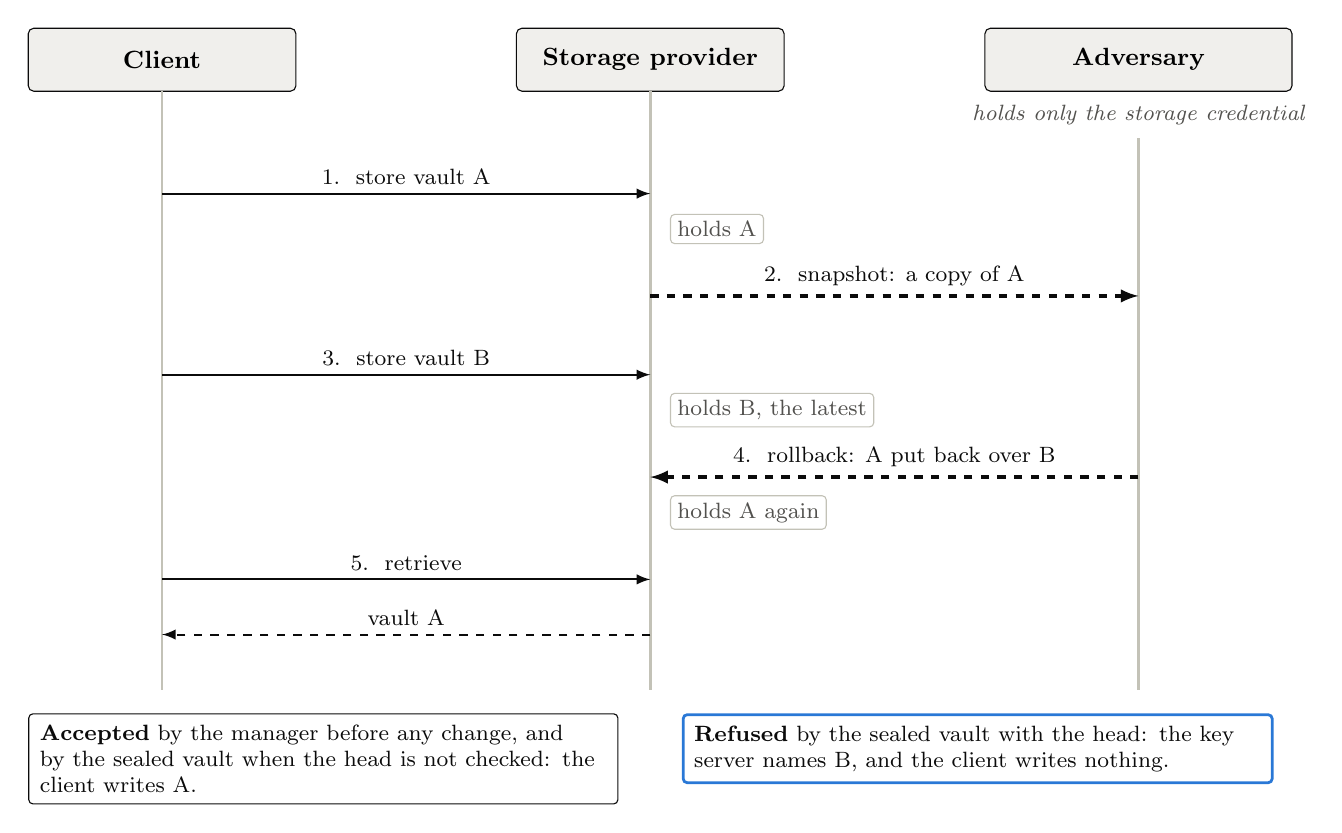
\begin{tikzpicture}
% the three parties and their lifelines
\node[party] (C) at (0,0)    {Client};
\node[party] (D) at (6.2,0)  {Storage provider};
\node[party, minimum width=3.9cm] (A) at (12.4,0) {Adversary};
\node[side, anchor=north, align=center] at (12.4,-0.45) {holds only the storage credential};
\foreach \x in {0,6.2} \draw[life] (\x,-0.4) -- (\x,-8.0);
\draw[life] (12.4,-1.0) -- (12.4,-8.0);
% what the storage provider holds, after each step
\newcommand{\state}[2]{\node[holds, anchor=west] at (6.45,#1) {#2};}
% 1 store A
\draw[msg] (0,-1.7) -- node[lab, above] {1.\ \ store vault A} (6.2,-1.7);
\state{-2.15}{holds A}
% 2 snapshot
\draw[bad] (6.2,-3.0) -- node[lab, above] {2.\ \ snapshot: a copy of A} (12.4,-3.0);
% 3 store B
\draw[msg] (0,-4.0) -- node[lab, above] {3.\ \ store vault B} (6.2,-4.0);
\state{-4.45}{holds B, the latest}
% 4 rollback
\draw[bad] (12.4,-5.3) -- node[lab, above] {4.\ \ rollback: A put back over B} (6.2,-5.3);
\state{-5.75}{holds A again}
% 5 retrieve
\draw[msg] (0,-6.6) -- node[lab, above] {5.\ \ retrieve} (6.2,-6.6);
\draw[rep] (6.2,-7.3) -- node[lab, above] {vault A} (0,-7.3);
% the outcomes
\node[outcome, anchor=north west, text width=7.2cm, align=left] at (-1.7,-8.3)
  {\textbf{Accepted} by the manager before any change, and by the sealed vault when the head is not checked: the client writes A.};
\node[outcome, anchor=north west, text width=7.2cm, align=left, draw=head, line width=1.0pt] at (6.6,-8.3)
  {\textbf{Refused} by the sealed vault with the head: the key server names B, and the client writes nothing.};
\end{tikzpicture}
\end{document}
